\subsection{Synthesizer}

\schematicpage{3}{Synth}

In order to generate the test signals, a pair of sinusoids at anywhere from
1~kHz to above 150~MHz, the instrument uses a sophisticated
high-speed Direct Digital Synthesis (DDS) integrated circuit.

\begin{figure}[H]
\centering
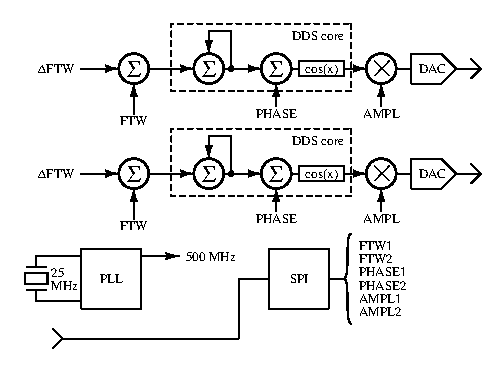
\includegraphics{too/dds}
\caption{DDS architecture}
\label{fig:dds}
\end{figure}

Figure~\ref{fig:dds} shows the internal architecture of the chip, somewhat
simplified from the version in the datasheet~\cite{ad9958}. In each of the two
independent waveform generators, a `frequency tuning word' (a 32-bit unsigned
integer) is repeatedly added to an accumulator at a rate of 500~MHz.
This causes the accumulator to increment, and overflow, at a higher rate for
higher tuning words. This sum is added to a phase offset, which allows each
signal to be independently offset from the other. This constantly incrementing
and resetting count is applied to a lookup table loaded with cosine values,
converting it from a digital ramp to a digital sinusoid. It is next multiplied
by an amplitude control value, and loaded into a digital-to-analog converter
(DAC) to generate the analog, sinusoidal waveform.

This integrated circuit is intended for radio applications. As such, it has
advanced features that this instrument does not require. It can be supplied
externally with a stable 500~MHz clock signal from a high quality
clock generator, but because we do not require such extreme stability, we
are instead using its internal Phase-Locked Loop (PLL) to multiply the clock
signal from a 25~MHz quartz crystal, \refdes{X1}, up to the full
internal clock frequency. Also, the device can generate modulated waveforms
using a 4-bit digital modulation input; these inputs are not used.

\subsection{Synthesizer Output Amplifiers}
\schematicpage{3}{Synth}

As is often the case with high-speed integrated circuits, the DDS chip has a
peculiar output system.

\begin{figure}[H]
\centering
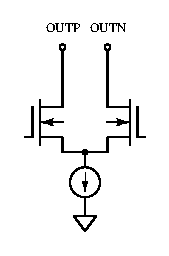
\includegraphics{too/dds-output}
\caption{DDS output circuit}
\label{fig:ddsoutput}
\end{figure}

The outputs are symmetric current sinks, which pull up to 9.9~mA
down from AVDD (1.8~V), and the voltage that appears at these
outputs must not deviate by more than 500~mV from AVDD (or else
the signal will distort severely). The intended application is for these
to be connected to a center-tapped transformer, with the center tap connected
to AVDD. This is impractical due to the frequency range required: any
transformer with a high enough inductance to operate at 1~kHz has
too much parasitic capacitance to operate at 150~MHz. Instead,
a DC-coupled differential amplifier was used, with carefully designed
termination networks to provide the correct voltage range.

\begin{figure}[H]
\centering
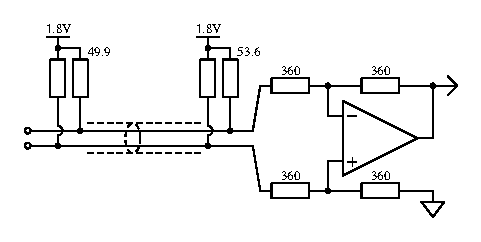
\includegraphics{too/dds-outamp}
\caption{Output amplifier for synthesizer}
\label{fig:synthoutput}
\end{figure}

The 49.9~\Ohm{} resistors terminate the transmission line at the
source. The amplifier's inputs are relatively low impedance, so 53.6~\Ohm{}
resistors were used as load termination to provide a more accurate impedance when
placed in parallel with the differential amplifier.

Note that the input impedances of the two sides of the differential amplifier
are not equal. On the side entering the noninverting (`positive') input, the
impedance to ground is the sum of the two input resistors, or 720~\Ohm{}.
However, on the other side, the end of the feedback chain is not grounded, it is
a 180\dg{} phase-shifted copy of the input signal. The equivalent input impedance
here is only 360~\Ohm{}, and a more proper termination resistor there
would be 57.6~\Ohm{}. However, these transmission lines are very short,
and the difference in impedance does not make a significant difference. Using
two different resistors here would have increased the design complexity and cost,
and was deemed unnecessary. 
    
